\section{Cloud-native data architecture}

\subsection{Decoupled storage and compute} 
Traditional data processing systems were designed under the assumption that storage and compute reside on the same node, with each node processing only the data it stores locally. This tight coupling forces the two layers to scale together, even when demand for each grows at different rates \parencite{dageville2016_snowflake_elastic_data_warehouse}.

Cloud architectures decouple these layers, placing data in object storage (a network-accessible store where data is identified by a unique key) \parencite{calder2011_windows_azure_storage,mesnier2003_object_based_storage} and provisioning compute resources independently and on demand, as illustrated in Figure~\ref{fig:storage-compute-architectures}. Object storage is inexpensive and effectively unbounded in capacity; however, it lacks query capabilities. The separation allows storage and compute to be scaled, priced, and allocated independently \parencite{pang2024_storage_disaggregated_databases}, and compute can be shut down entirely when idle \parencite{dageville2016_snowflake_elastic_data_warehouse}. Multiple engines can also read the same underlying data without coordination through a shared server \parencite{pang2024_storage_disaggregated_databases}. \textcite{dageville2016_snowflake_elastic_data_warehouse} note that this arrangement incurs higher latency and Central Processing Unit (CPU) overhead per request than a node in which compute and storage are tightly coupled, making format design critical: formats that minimize the volume of data read per query gain a clear advantage.

\begin{figure}[H]
    \centering
    \subfloat[Coupled storage and compute.\label{fig:coupled-compute}]{%
        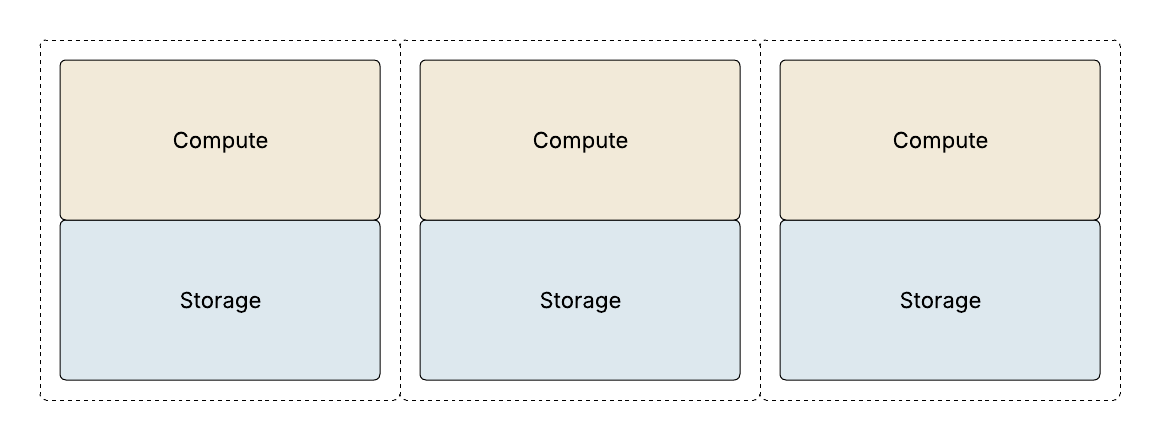
\includegraphics[valign=t, width=0.45\textwidth]{Chapters/02-background/sub-chapters/figures/02-coupled-compute.png}%
    }
    \hfill
    \subfloat[Decoupled storage and compute.\label{fig:decoupled-compute}]{%
        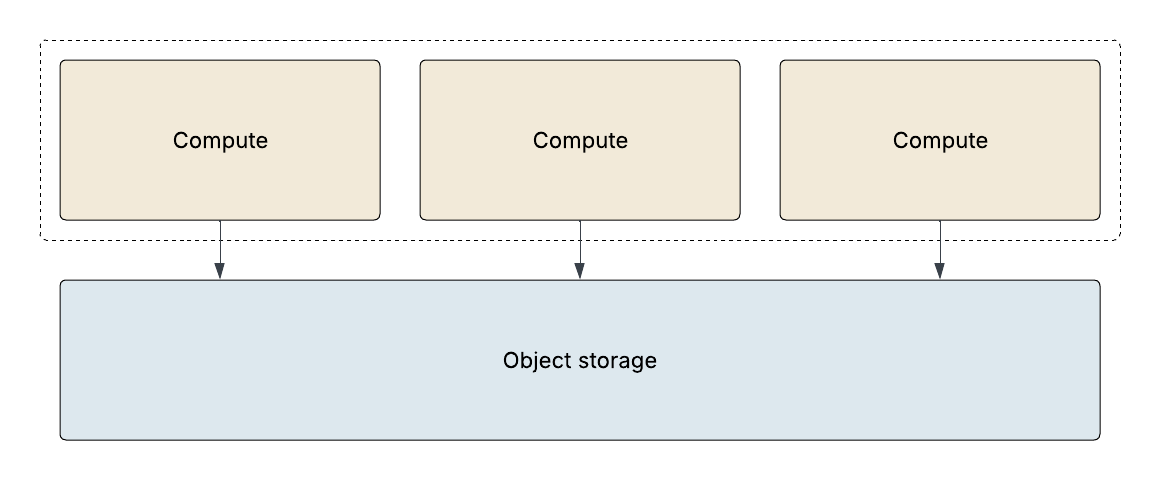
\includegraphics[valign=t, width=0.45\textwidth]{Chapters/02-background/sub-chapters/figures/02-decoupled-compute.png}%
    }
    \caption[Coupled versus decoupled storage and compute architectures.]{Comparison of storage and compute architectures. (a) In the traditional coupled architecture, each node bundles its own compute and storage, so the two layers must scale together as a unit. (b) In the decoupled architecture, multiple independent compute resources access a shared object storage layer, allowing storage and compute to be provisioned, priced, and scaled independently of one another.}
    \label{fig:storage-compute-architectures}
\end{figure}

\subsection{Object storage and HTTP access}
Object storage is the shared layer underlying these architectures. It organizes data as opaque objects identified by a key within a flat container namespace, accessed via a network \acrfull{api} rather than \acrshort{posix} file system calls \parencite{mesnier2003_object_based_storage, calder2011_windows_azure_storage}. Commercial implementations such as Azure Blob Storage expose each object as a \acrfull{https} \acrfull{url} accessed over \acrfull{http} \parencite{microsoft2024_azure_blob_introduction}.

Read access is mediated by \acrshort{http} itself. \textcite{fielding2022_rfc9110_http_semantics} standardizes the \texttt{Range} request header, which allows a client to retrieve an arbitrary byte interval of a remote resource without downloading the whole file. Operational experience confirms the viability of this access model for analytical workloads at scale \parencite{vuppalapati2020_snowflake_elastic_query_engine, durner2023_exploiting_cloud_object_storage}. Cloud-native data formats are designed around this access pattern: layout metadata is placed at a known offset within the object so that readers can fetch it first, after which range requests retrieve only the byte intervals required by the query \parencite{maso2023_ogc_cog_standard}, as illustrated in Figure~\ref{fig:http-range-requests}.

\begin{figure}[H]
    \centering
    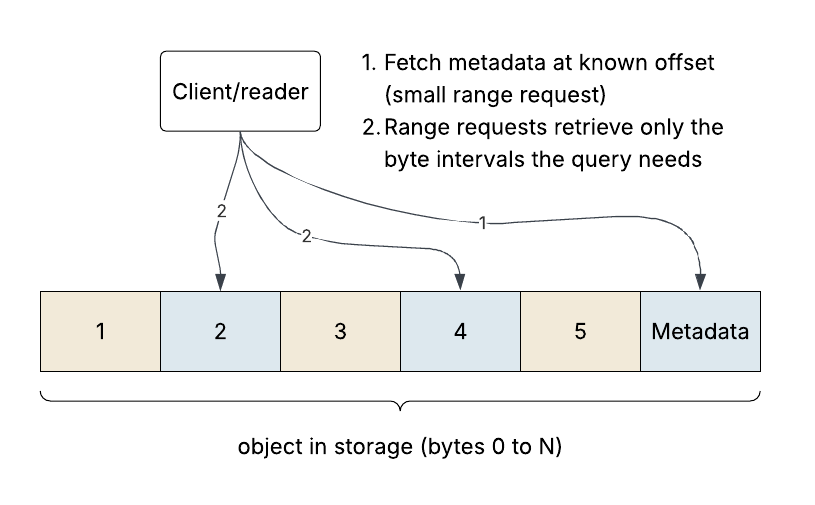
\includegraphics[width=0.85\textwidth]{Chapters/02-background/sub-chapters/figures/02-http-range-requests.png}
    \caption[HTTP range request access pattern.]{HTTP range request access pattern for cloud-native objects. The reader first issues a small range request for the metadata block at a known offset within the object (1), parses the layout information it returns to identify which byte intervals satisfy the query, and then issues range requests for only those intervals (2). Bytes outside the requested intervals are never transferred.}
    \label{fig:http-range-requests}
\end{figure}

\subsection{Distributed and non-distributed computation}
\label{sec:distributed-and-non-distributed-compute}
With storage and compute decoupled, the choice of computational model becomes a central architectural decision. Under the non-distributed model, a query executes entirely within a single process on one node, with no coordination overhead between workers \parencite{mcsherry2015_scalability_but_at_what_cost}. Under the distributed model, by contrast, both data and computation are split across multiple worker nodes coordinated by a driver or scheduler (a central process that assigns tasks to workers and aggregates their results) \parencite{stonebraker1986_case_for_shared_nothing,zaharia2012_resilient_distributed_datasets}. Figure~\ref{fig:compute-models} contrasts the two models.

\begin{figure}[H]
    \centering
    \subfloat[Non-distributed compute.\label{fig:non-distributed-compute}]{%
        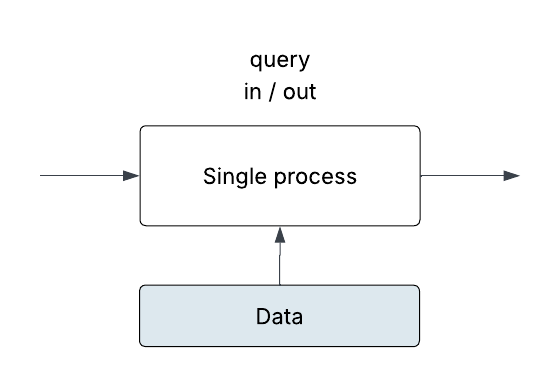
\includegraphics[valign=t, width=0.45\textwidth]{Chapters/02-background/sub-chapters/figures/02-non-distributed-compute.png}%
    }
    \hfill
    \subfloat[Distributed compute.\label{fig:distributed-compute}]{%
        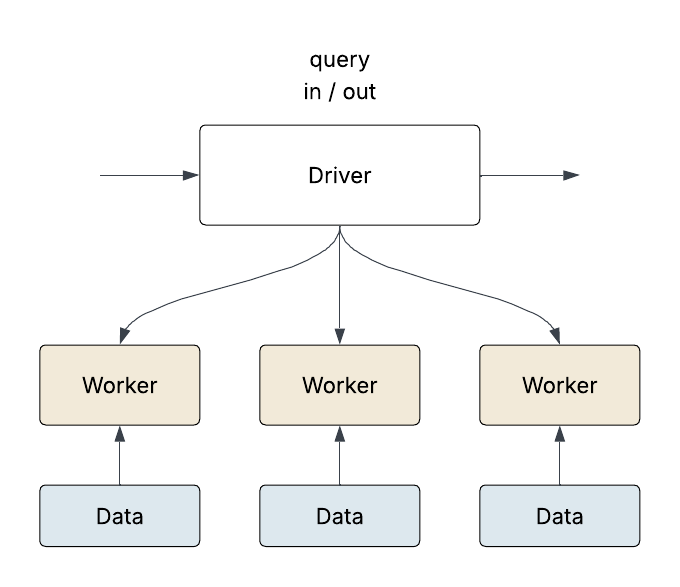
\includegraphics[valign=t, width=0.45\textwidth]{Chapters/02-background/sub-chapters/figures/02-distributed-compute.png}%
    }
    \caption[Non-distributed versus distributed compute models.]{Comparison of compute models. (a) In the non-distributed model, a single process executes the query end-to-end, with no coordination overhead between workers. (b) In the distributed model, a driver dispatches tasks to multiple workers, each operating on a partition of the data.}
    \label{fig:compute-models}
\end{figure}

This distribution introduces overhead: task scheduling, data shuffling between nodes (the network-based redistribution of intermediate data), serialization, and network communication between workers all add latency before any computation begins \parencite{mcsherry2015_scalability_but_at_what_cost,zaharia2012_resilient_distributed_datasets}. Consequently, distributed systems outperform single-node systems only when the dataset or computation is large enough to justify the coordination cost \parencite{mcsherry2015_scalability_but_at_what_cost}. For spatial workloads in particular, the data partitioning strategy is critical: poor spatial partitioning leads to skewed workloads in which some workers process far more data than others, degrading parallel efficiency \parencite{tang2020_locationspark_distributed_spatial_query}.

\subsection{Cloud cost model}
The choice between distributed and non-distributed compute is ultimately governed by a cost model in which every resource---storage, processing, and bandwidth---is separately metered \parencite{mell2011_nist_definition_of_cloud_computing}. In practice, this metering takes the form of a pay-as-you-go model in which compute and storage are acquired on a short-term basis and released when no longer needed \parencite{armbrust2010_view_of_cloud_computing}. Each resource carries its own pricing dimension: compute is billed for allocated virtual cores in per-minute increments \parencite{microsoft2024_virtual_machines_pricing}; object storage is priced per gigabyte-month across access tiers, with transactional APIs charged per $10,000$ operations \parencite{microsoft2024_azure_data_lake_storage_pricing}; and outbound network traffic is billed per gigabyte of egress \parencite{microsoft2024_bandwidth_pricing}. To dampen the volatility of on-demand pricing, providers also offer reserved instances that trade flexibility for lower rates over one- or three-year commitment terms \parencite{microsoft2024_azure_reservations}. Elasticity (the ability to provision and release resources rapidly to match demand \parencite{mell2011_nist_definition_of_cloud_computing}), therefore, has direct cost implications: serverless platforms charge only for active execution time and scale to zero when idle, whereas long-running clusters continue to accrue charges regardless of utilization \parencite{jonas2019_berkeley_view_on_serverless_computing}.